\documentclass[12pt,a4paper,fleqn]{article}
\usepackage{rmpackages}																% usual packages
\usepackage{rmtemplate}																% graphic charter
\usepackage{rmexocptce}																% for DS with cptce eval

%\cfoot{} 													% if no page number is needed
%\renewcommand\arraystretch{1.5}		% stretch table line height

\newcommand{\prog}{\textcolor{red}{PROGRAMME}}

\usepackage{pdflscape}

\begin{document}

\begin{header}
Chapitre 9 -- Spectres d'émission
\end{header}

Ce document présente l'ensemble de la séquence sur les spectres d'émission.
Cette séquence s'intègre dans la partie \og Optique \fg{} du thème \og Ondes et signaux \fg{} du programme de seconde.
La séance correspondant à la visite d'aujourd'hui mercredi 5 mai 2021 est indiquée en \textcolor{bleu_f}{bleu} ci-dessous.

\section*{Aperçu de la séquence}

\subsection*{Semaine du 3 mai}

\begin{itemize}
\item[•] \textbf{Présentiel (groupe 2) :}
\begin{itemize}
\item Séance 1 (TP) : obtenir des spectres et les exploiter. L'accent est porté sur les spectres d'émission de raies.
\item Séance 2 (Cours) : rappels sur la lumière, vitesse.
\textcolor{bleu_f}{\item Séance 3 (Activité) : spectre du rayonnement émis par un corps chaud.}
\end{itemize}
\item[•] \textbf{Distanciel (groupe 1) :}
\begin{itemize}
\item Classe virtuelle courte pour présenter le thème et le travail de la semaine.
\item Quiz QuiZinière : obtention de spectres et spectres de raies.
\item Défis confinés : spectre du rayonnement émis par un corps chaud.
\end{itemize}
\end{itemize}

\subsection*{Semaine du 10 mai}
\begin{itemize}
\item[•] \textbf{Distanciel (groupes 1 et 2) :}
\begin{itemize}
\item Évaluation sommative QuiZinière.
\item Défis confinés : un spectroscope maison.
\end{itemize}
\end{itemize}

\section*{Suite de la progression}

La séquence suivante portera sur les lentilles.

\section*{Légende}

Même si elles ne sont pas systématiquement évaluées, les compétences de la démarche scientifique mobilisées à chaque étape sont identifiées par le code suivant :
\begin{itemize}
\item[(•] \rco{} : Mobiliser ses connaissances)
\item[•] \app{} : S'approprier
\item[•] \anarai{} : Analyser, raisonner
\item[•] \rea{} : Réaliser
\item[•] \val{} : Valider
\item[•] \com{} : Communiquer
\end{itemize} 





\newpage
\section*{Séance 1 : TP -- Spectres d'émission}

\noindent
\prog{} :
\begin{itemize}
\item[•] (Notion) Spectres d'émission : spectres continus d'origine thermique, \textit{spectres de raies}.
\item[•] (Notion) Longueur d'onde dans le vide ou dans l'air.
\item[•] (Capacité expérimentale) Produire et exploiter des spectres d'émission obtenus à l'aide d'un système dispersif et d'un analyseur de spectre.
\end{itemize}

\subsection*{Différents types de spectres}

\begin{enumerate}
\item \app{} \anarai{}

Exploiter qualitativement les spectres de différentes sources lumineuses, distinguer les spectres continus des spectres de raies.

\prog{} : spectre continu, spectre de raies.

\end{enumerate}

\subsection*{Un nombre pour caractériser la \og couleur \fg{} d'une radiation}

\begin{enumerate}[resume]
\item \app{} \anarai{}

Lien entre la couleur de la lampe à vapeur de sodium et la longueur d'onde.

\prog{} : caractériser un rayonnement monochromatique par sa longueur d'onde [...].

\item \rea{} \val{}

Réalisation et exploitation du spectre de la lumière émise par une lampe à vapeur de sodium.

\prog{} : exploiter un spectre de raies.
\end{enumerate}

\subsection*{Que contient cette lampe ?}

\begin{enumerate}[resume]
\item \app{} \anarai{} \rea{} \val{} \com{}

Obtenir et exploiter le spectre de raies d'une lampe spectrale pour déterminer le gaz qu'elle contient, en mettant en œuvre les étapes de la démarche scientifique.

\textit{Aide : le document 3 du sujet est complété par les images des spectres de raies.}

\prog{} : exploiter un spectre de raies.
\end{enumerate}






\newpage
\section*{Séance 2 : Cours}

\noindent
\prog{} :
\begin{itemize}
\item[•] (Notion) Propagation rectiligne de la lumière.
\item[•] (Notion) Vitesse de propagation de la lumière dans le vide ou dans l'air.
\end{itemize}

\subsection*{Rappels}

\begin{itemize}
\item[•] \anarai

Source primaire, objet diffusant.

\item[•] \rea{}

Faire le schéma d'un faisceau laser.

\prog{} : propagation rectiligne de la lumière.
\end{itemize}

\subsection*{Vitesse de la lumière}

\begin{itemize}
\item[•] \app{} \rea{}

Calculer la vitesse de propagation de la lumière.

\prog{} : Vitesse de propagation de la lumière dans le vide ou dans l'air.

\item[•] \rea{}

Comparer la vitesse de la lumière à d'autres vitesses.

\prog{} : effectuer le quotient de deux grandeurs pour les comparer.

\prog{} : citer la valeur de la vitesse de la lumière dans le vide ou dans l'air et la comparer à d'autres vitesses couramment rencontrées.
\end{itemize}





\newpage

\section*{\textcolor{bleu_f}{Séance 3 : De quelle couleur sont les étoiles les plus chaudes ?}}

\prog :
\begin{itemize}
\item[•] Caractériser le spectre du rayonnement émis par un corps chaud, en mettant en œuvre les étapes de la démarche scientifique.
\end{itemize}

\subsection*{Évaluation formative et contextualisation (Plickers)}

\begin{center}
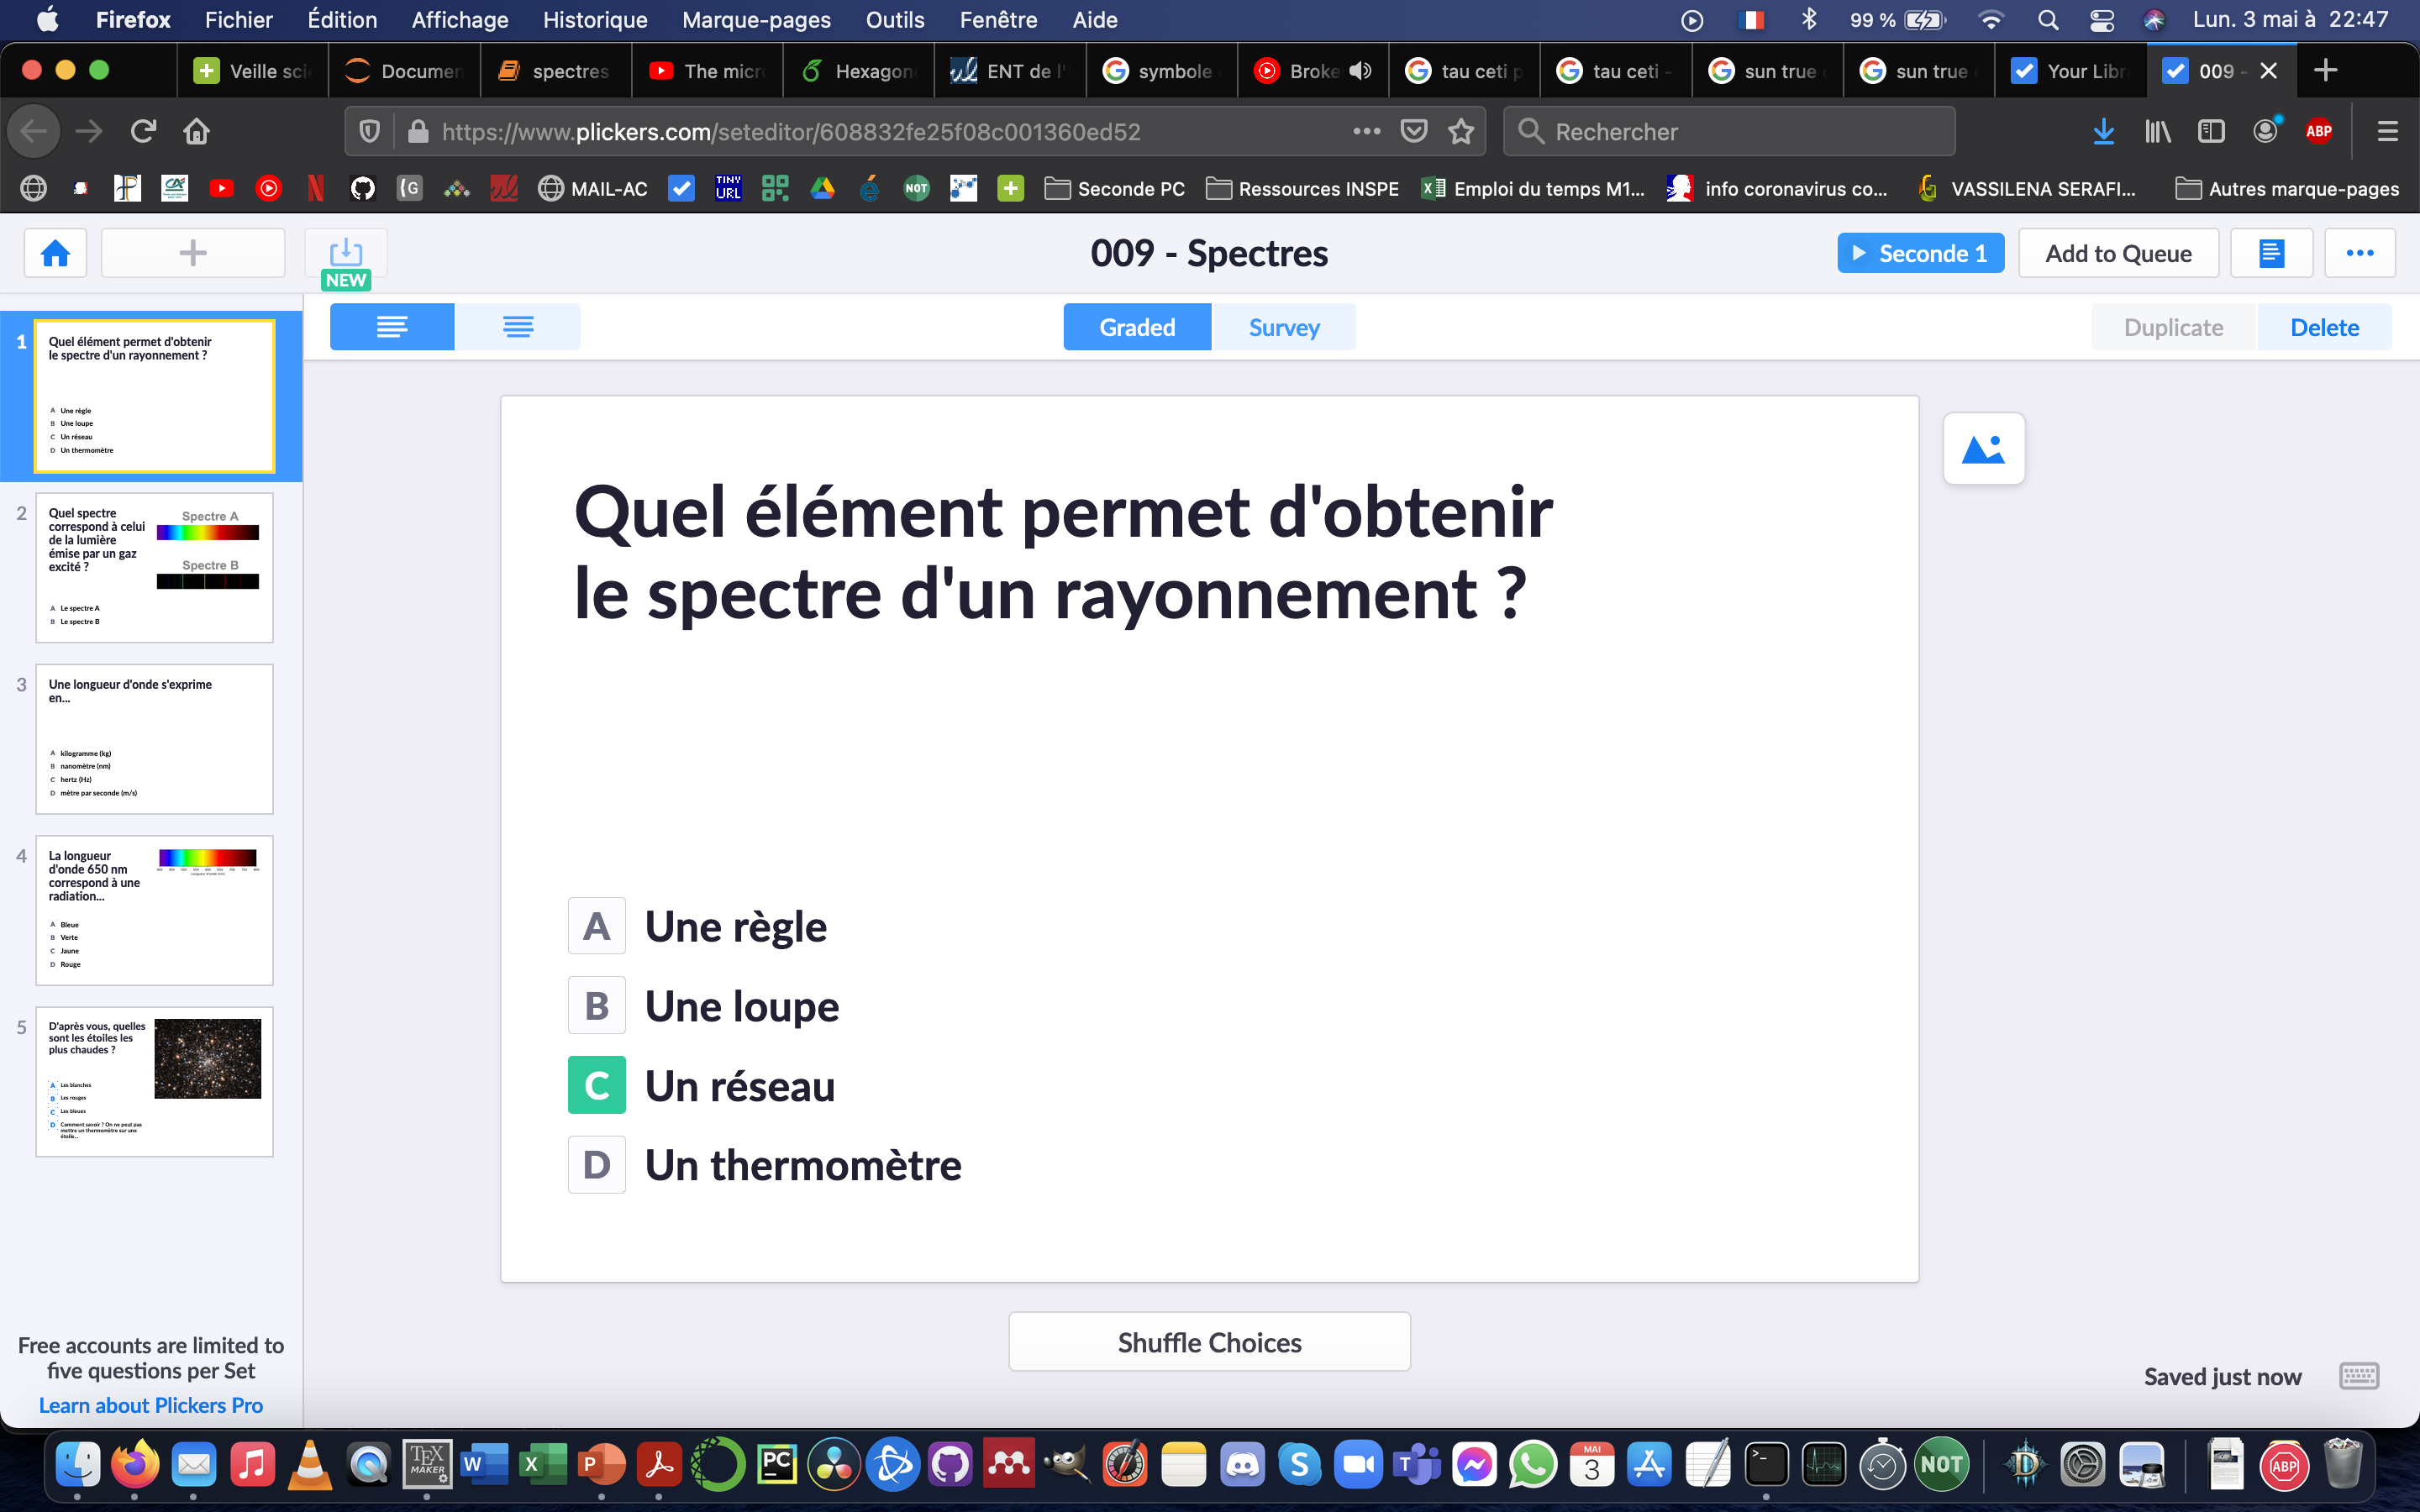
\includegraphics[trim=310 150 300 250,clip,width=.19\linewidth]{inspection/plickers1.png}
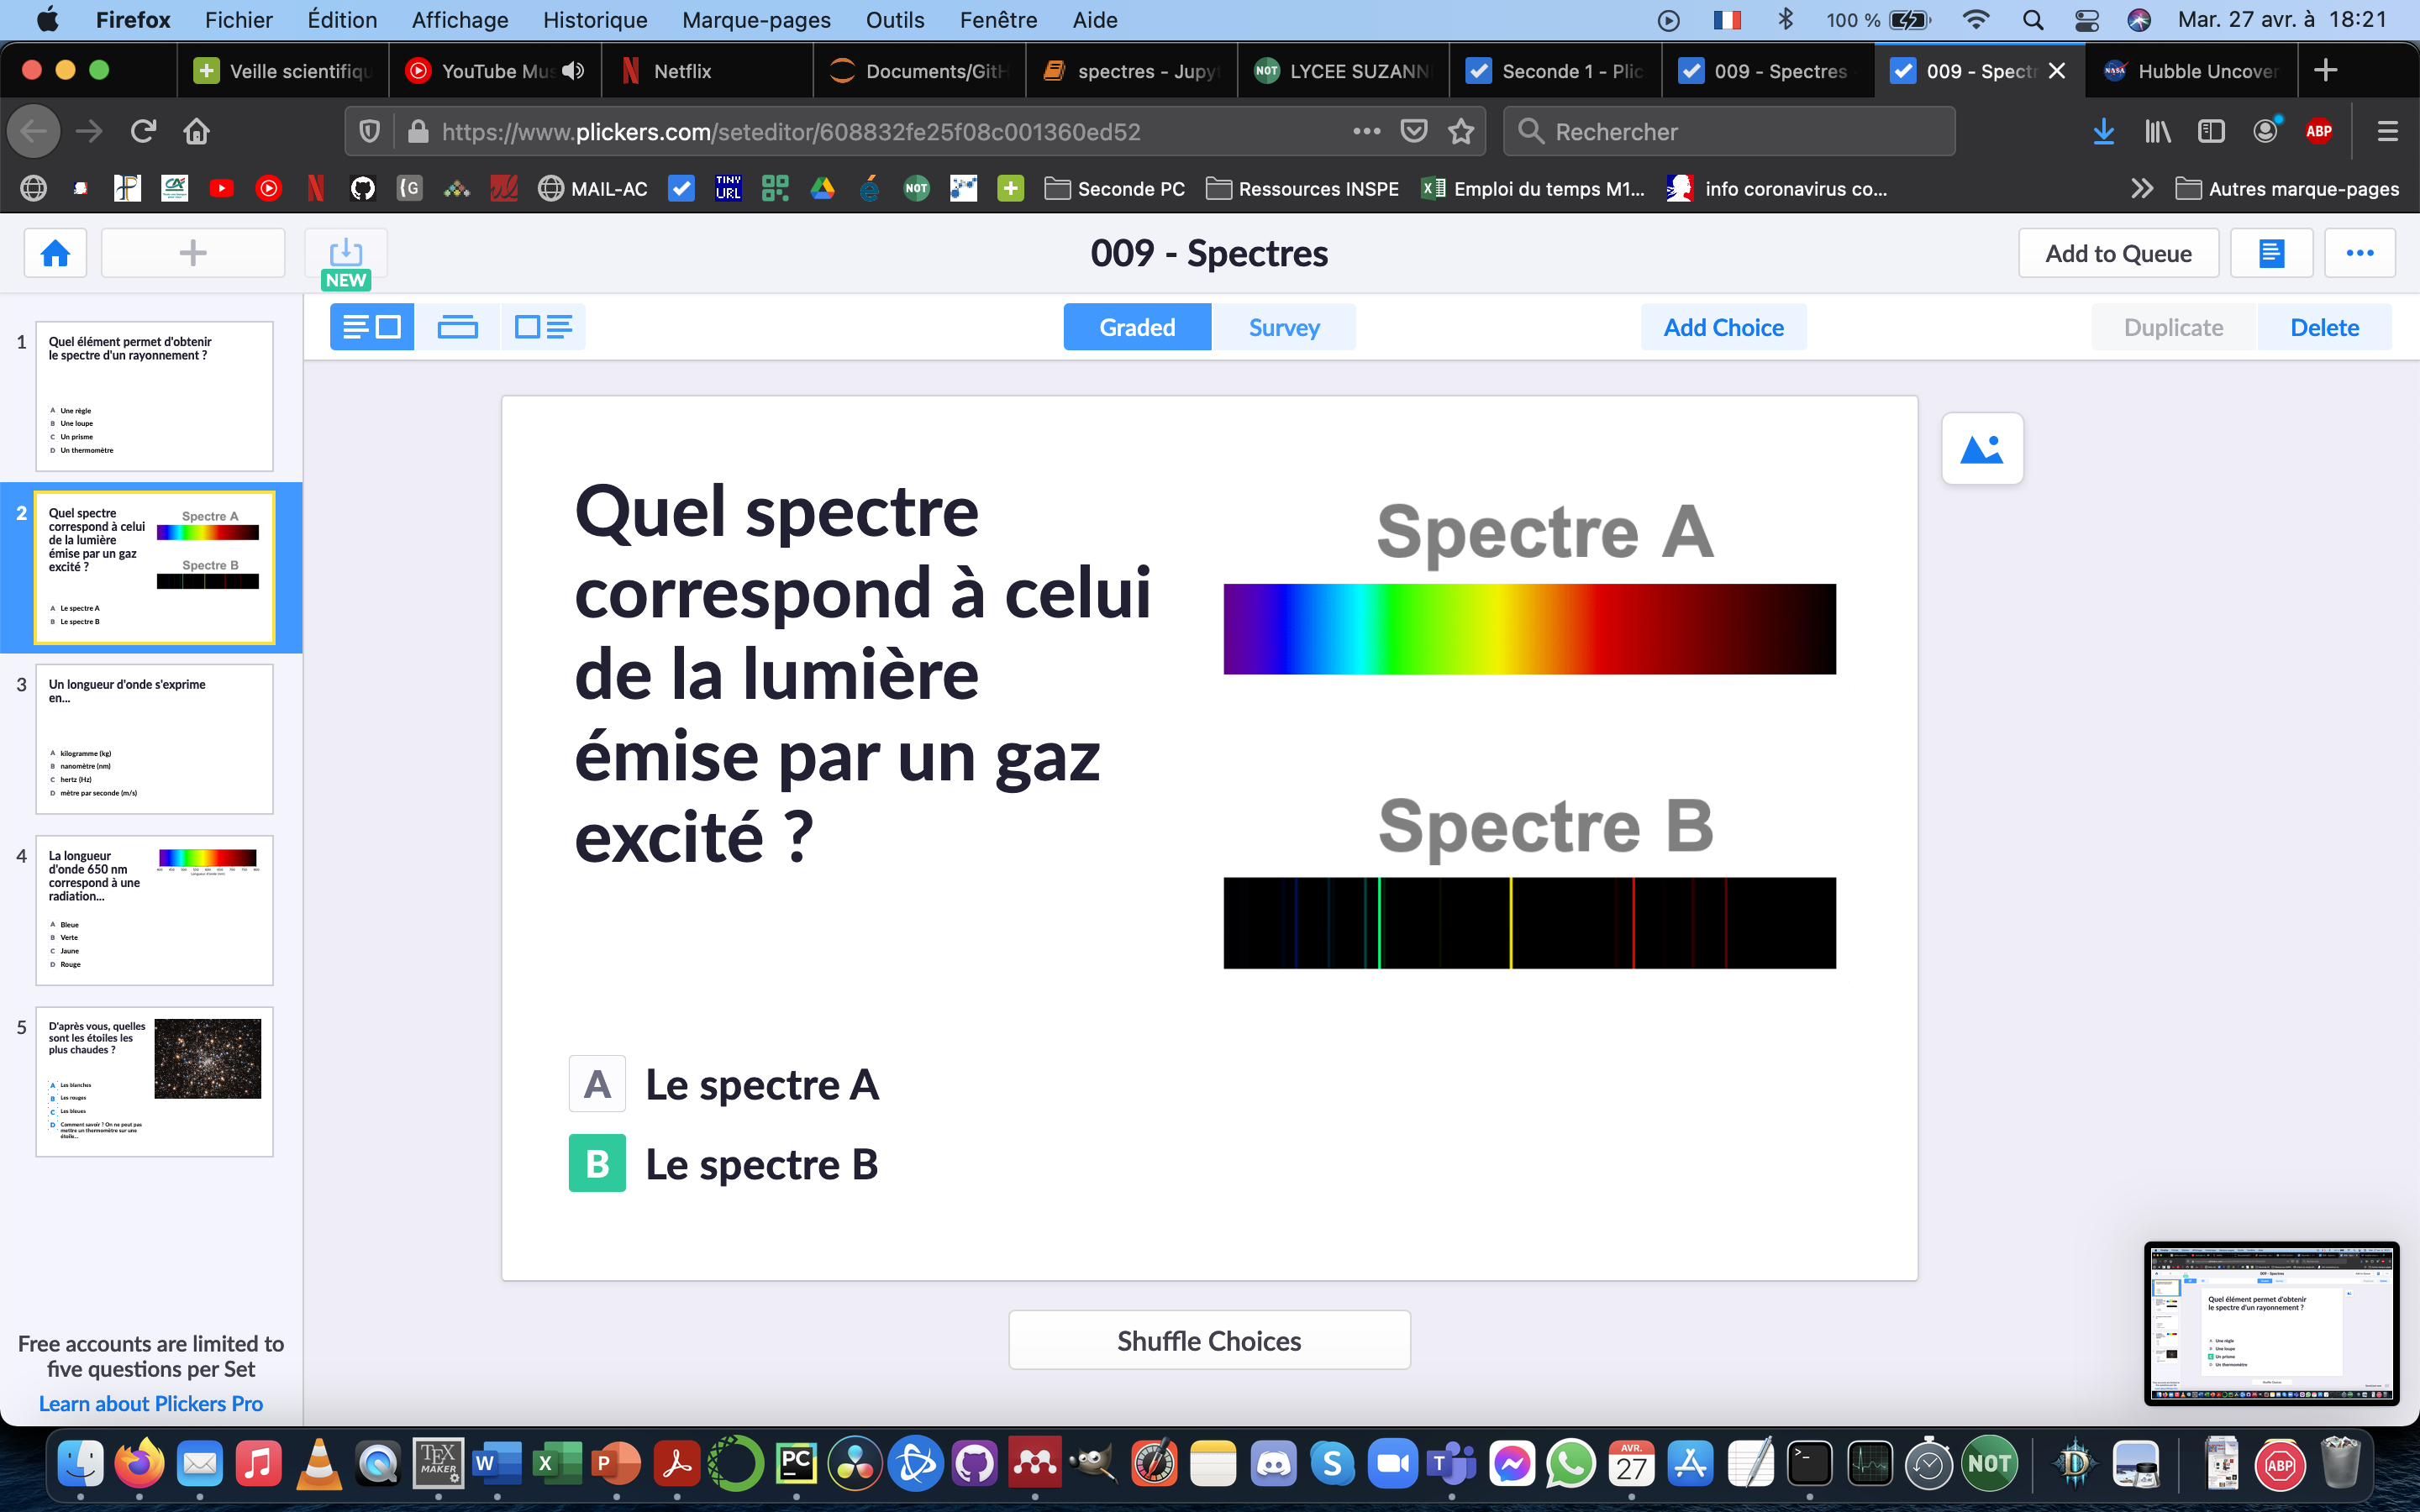
\includegraphics[trim=310 150 300 250,clip,width=.19\linewidth]{inspection/plickers2.png}
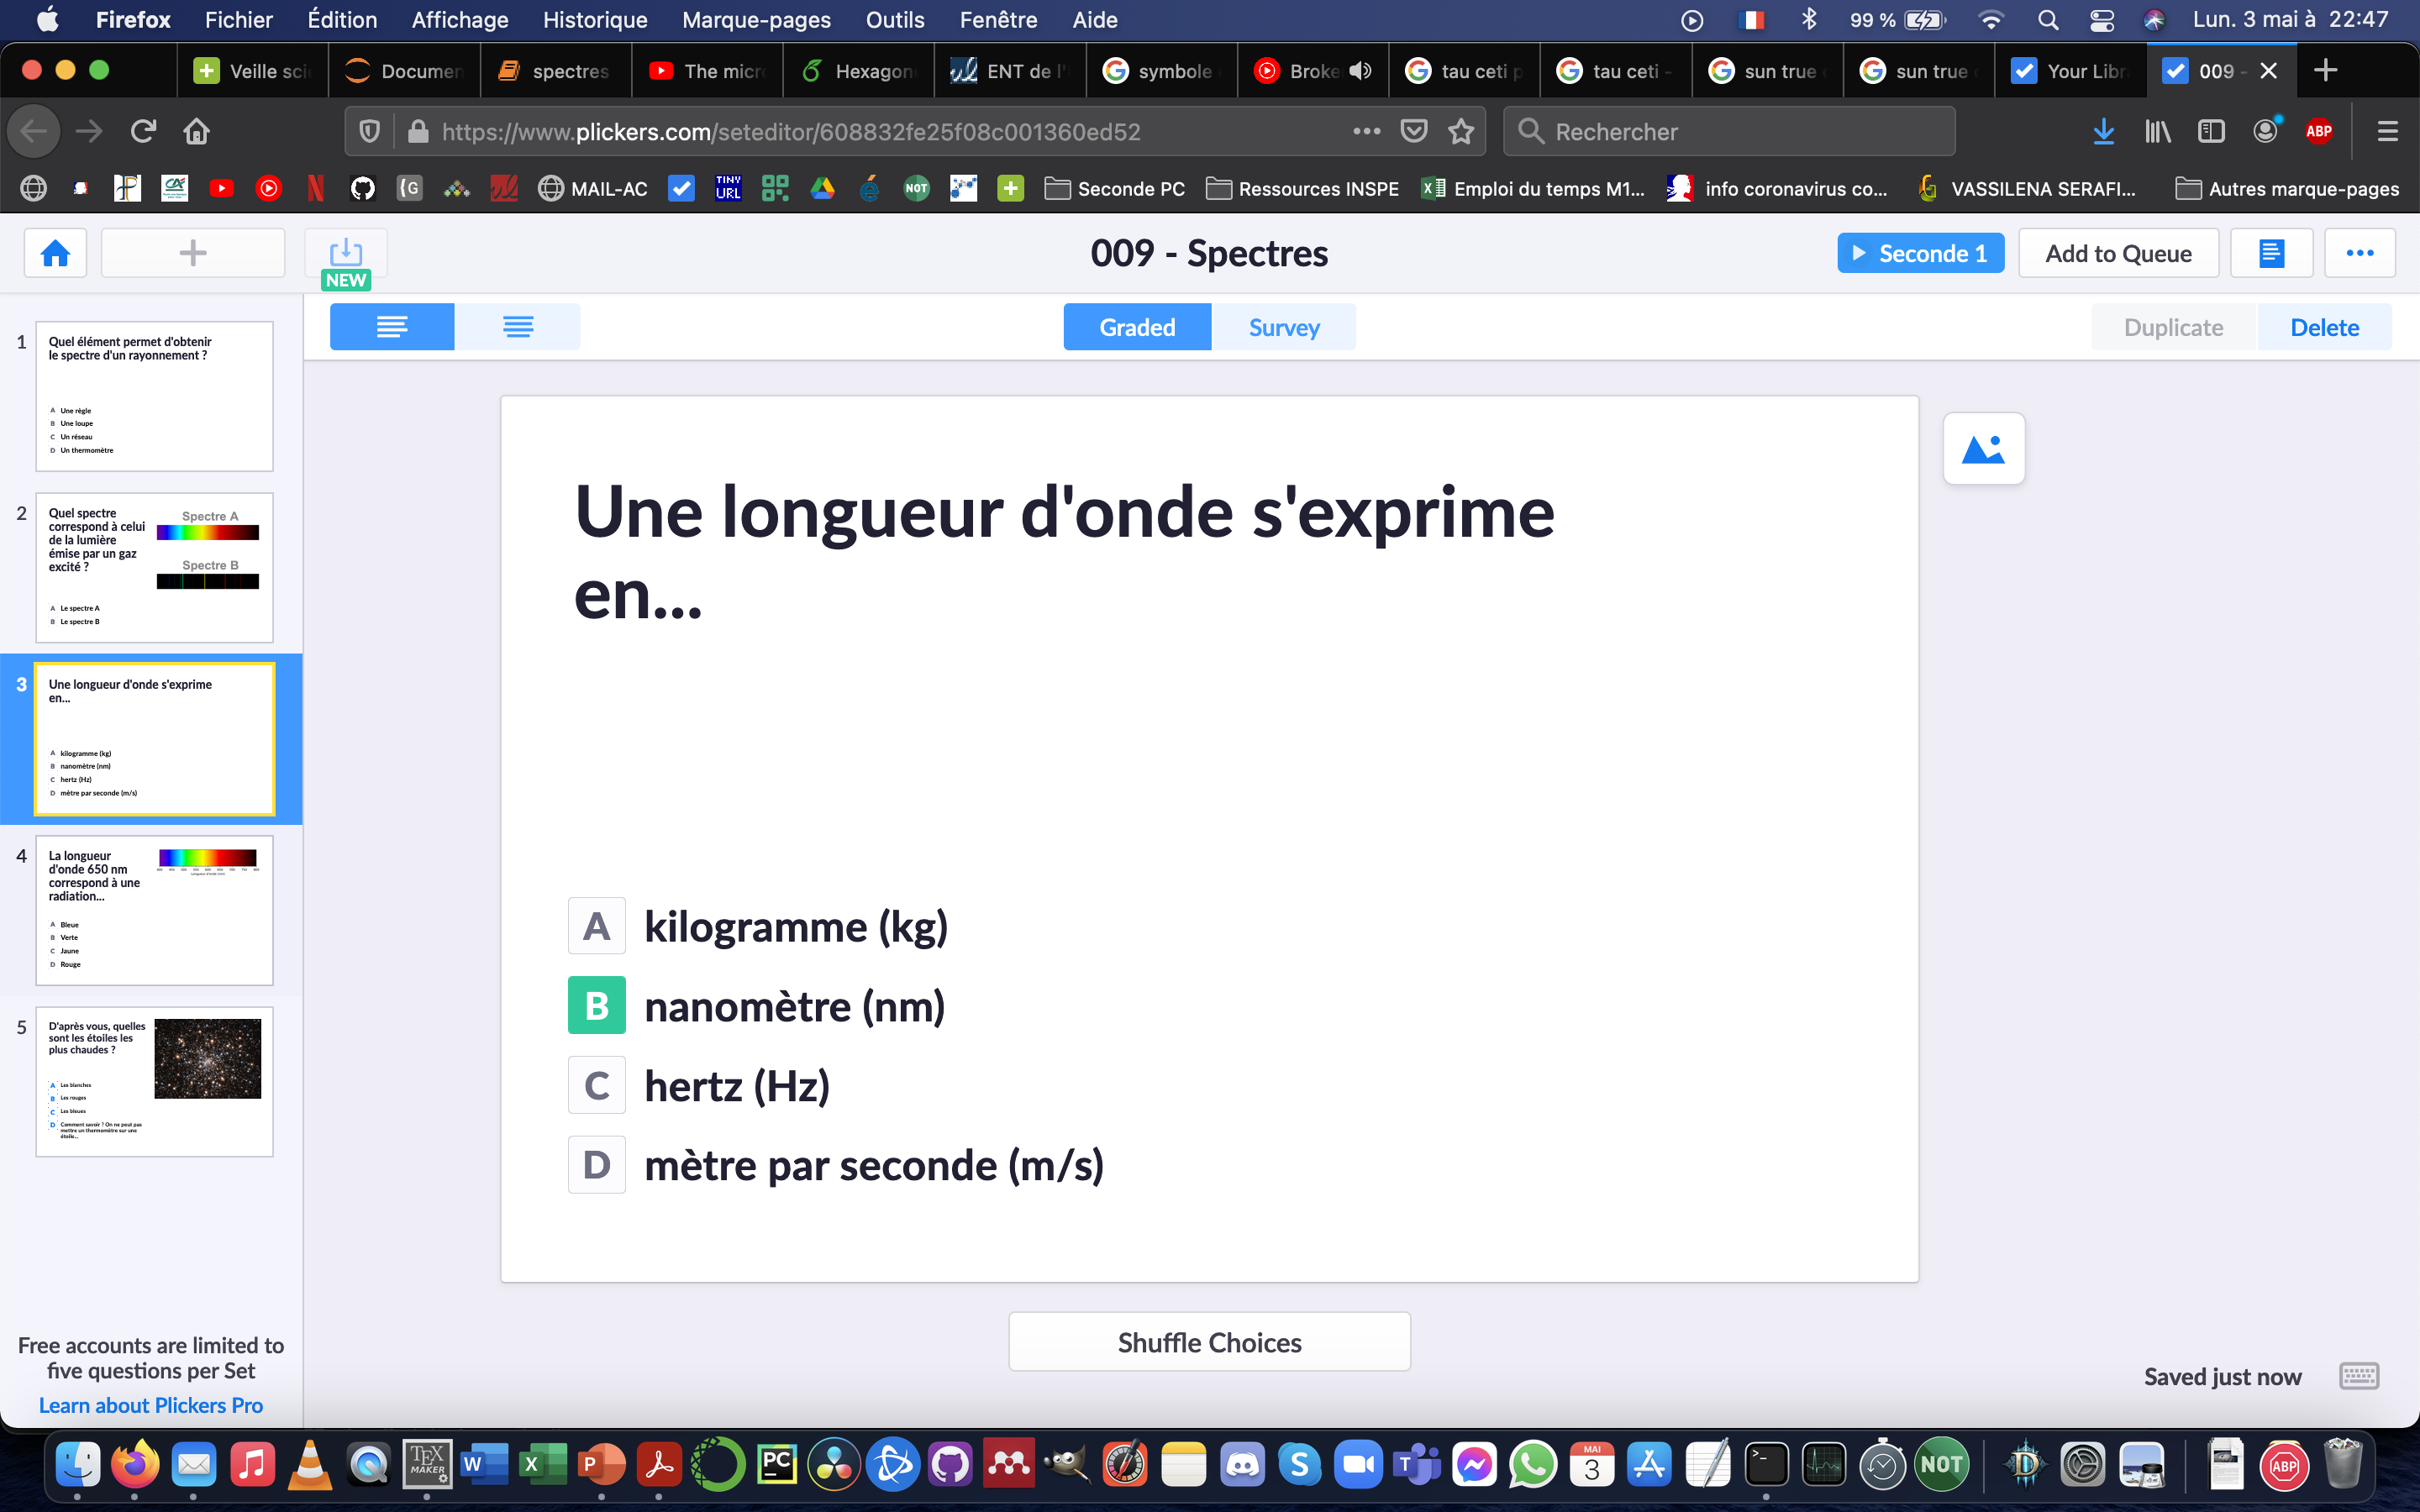
\includegraphics[trim=310 150 300 250,clip,width=.19\linewidth]{inspection/plickers3.png}
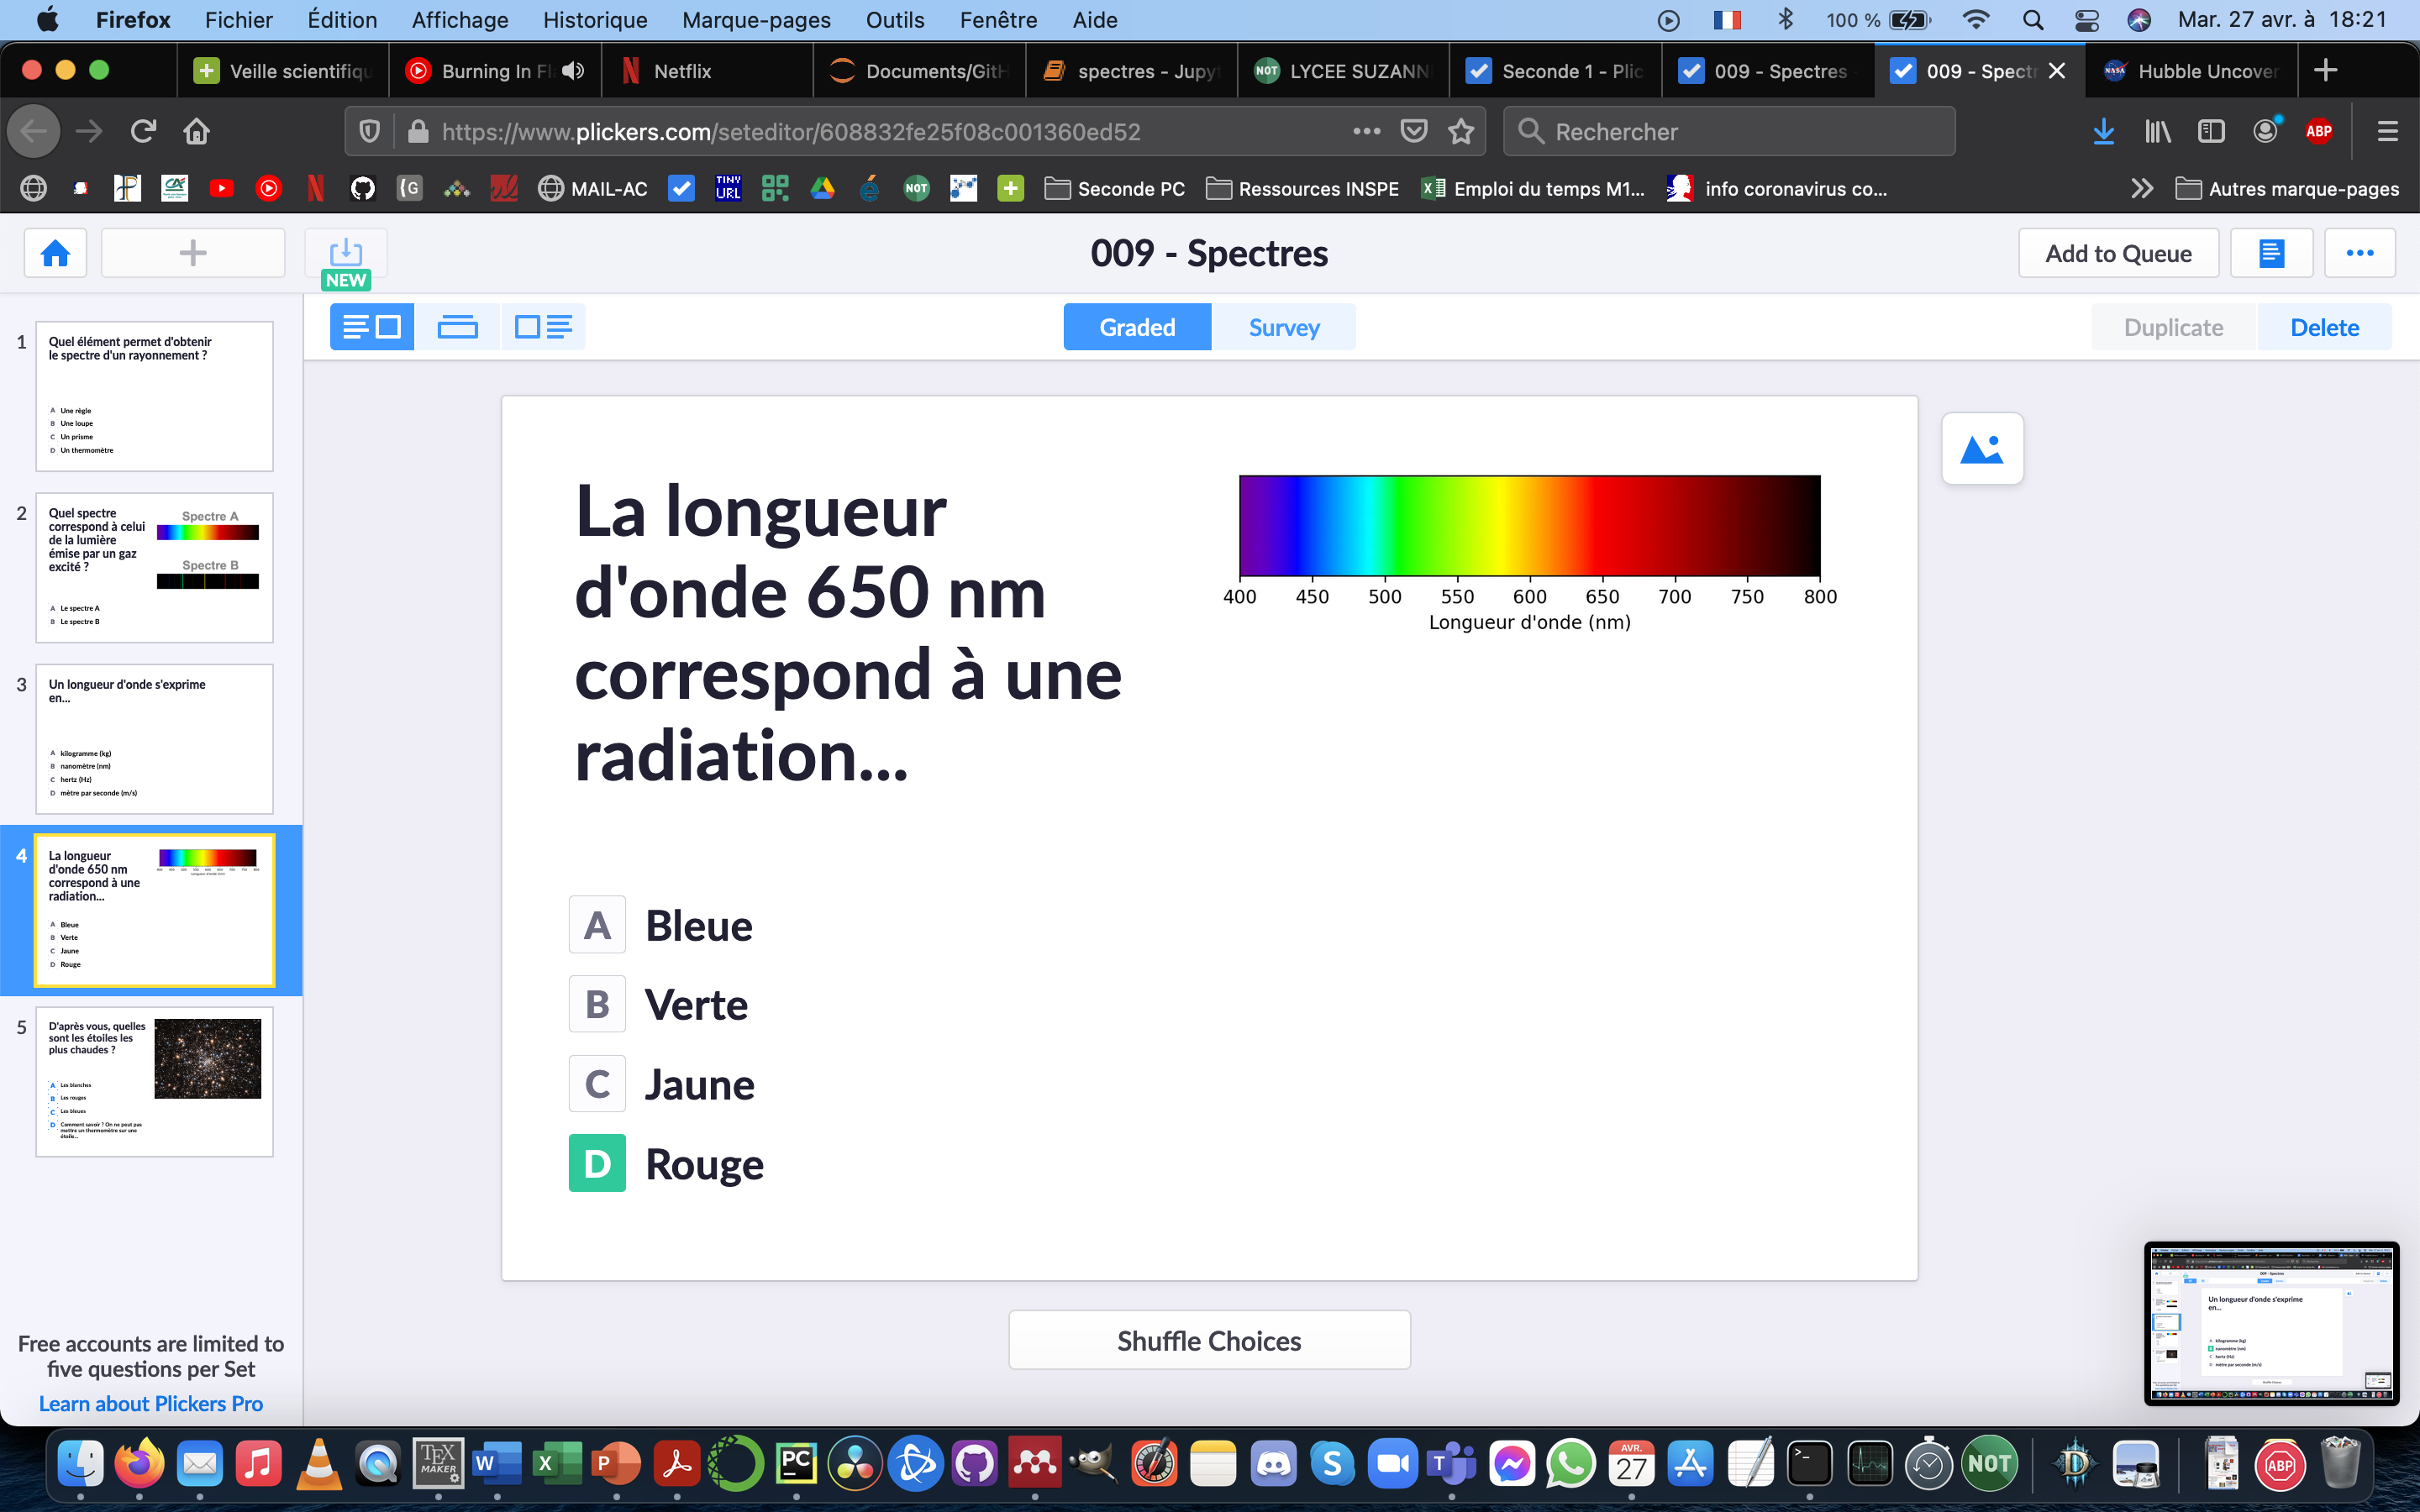
\includegraphics[trim=310 150 300 250,clip,width=.19\linewidth]{inspection/plickers4.png}
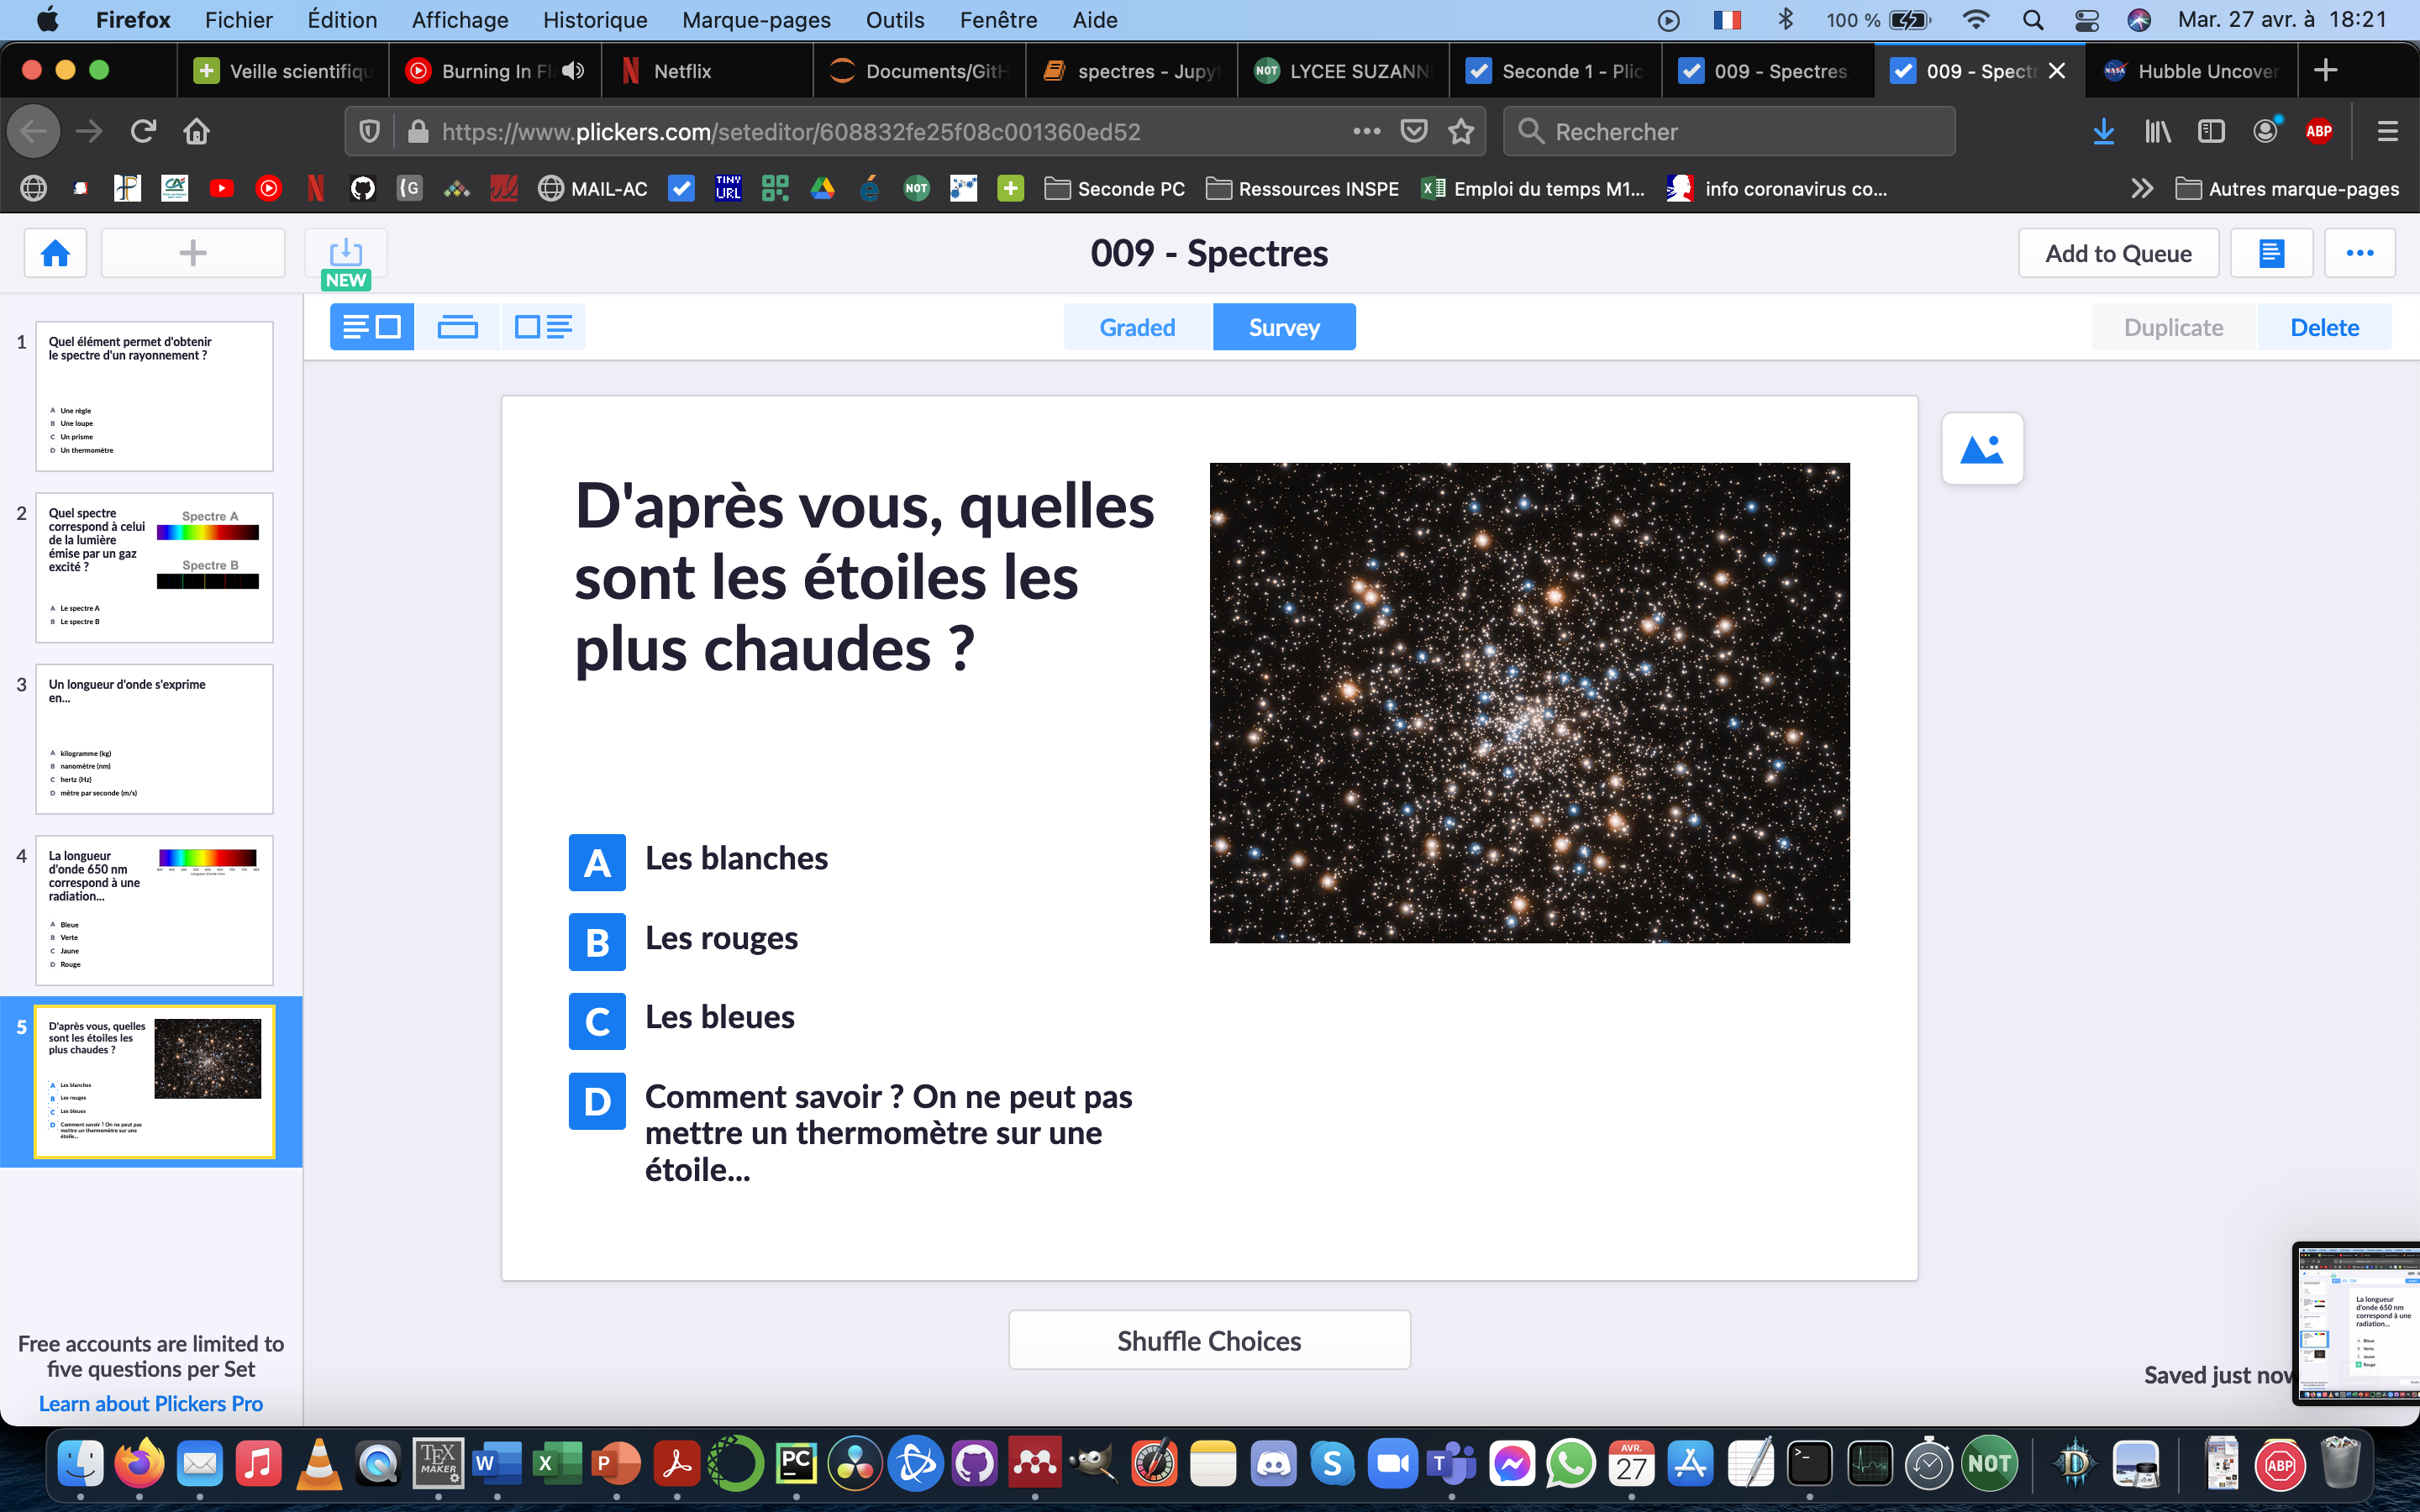
\includegraphics[trim=310 150 300 250,clip,width=.19\linewidth]{inspection/plickers5.png}
\end{center}

\subsection*{Activité}

\begin{enumerate}
\item \anarai{}

Quelles sont les étoiles les plus chaudes ?

Formuler et justifier une hypothèse sur la question, individuellement puis en groupe.

\item \rea{}

Schéma du spectroscope à réseau.

\textit{Aide : rappel des éléments nécessaires au montage.}

\prog : produire [...] des spectres...

\item \app{} \anarai{}

Spectres continus, enrichissement vers le bleu.
\begin{itemize}
\item[•] Version 1 : trouver la température associée à chaque spectre en exploitant les courbes.
\item[•] Version 2 : la température de chaque spectre est directement donnée.
\end{itemize}

\textit{Aide : attirer l'attention sur les extrémités du spectre, notamment en comparant le spectre obtenu à haute et \og basse \fg{}  température.}

\prog : caractériser le spectre du rayonnement émis par un corps chaud.

\item \anarai{}

Classer les étoiles en fonction de leur température d'après le spectre de leur rayonnement.

\textit{Aide : quelle couleur devient plus intense quand le corps chauffe ? Comparer avec les spectres précédents.}

\prog : caractériser le spectre du rayonnement émis par un corps chaud.

\item \val{}

Conclusion
\end{enumerate}

\subsection*{Supplément}

\begin{enumerate}[resume]
\item \app{} \anarai{}

Identifier le gaz  en arrière plan de la nébuleuse à tête de cheval d'après son spectre d'émission.

\prog{} : exploiter un spectre de raies.

\item \rco{} \rea{}

Calculer la distance à laquelle est située cette nébuleuse.

\prog{} : citer la valeur de la vitesse de la lumière dans le vide.
\end{enumerate}

\subsection*{Bilan}

\begin{enumerate}
\item[] \com{}

Faire un bilan oral de l'activité en reprenant les étapes de la démarche scientifique.

Conclusion dans le cours.
\end{enumerate}

\subsection*{Évaluation}

Trois compétences sont évaluées pendant la séance (la dernière pourra être évaluée à la séance suivante si le temps manque).

\begin{center}
\begin{tabular}{l|l|c}
\textbf{Compétence} & \textbf{Aptitude et observables} & \textbf{Niveau} \\
\hline \hline
\rea{}	& Réaliser un schéma correct d’un dispositif expérimental		& \\
			& Le schéma est clair, correspond à l'expérience et légendé 	& A \\
			& Un des items ci-dessus manquant											& B \\
			& Deux des items ci-dessus manquants										& C \\
			& Incapacité à réaliser le schéma													& D \\
\hline
\val{}	& Avoir un regard critique sur mes résultats								& \\
			& Conclusion pertinente avec une critique de l'hypothèse 		& A \\
			& Conclusion pertinente, sans critique de l'hypothèse				& B \\
			& La conclusion ne répond pas complètement à la question	& C \\
			& Absence de conclusion																& D \\
\hline
\com{}	& Rendre compte de façon orale													& \\
			& Évaluation suivant la grille spécifique (cf. ci-dessous	)			&
\end{tabular}
\vfill
\includegraphics[width=\linewidth, trim=8 5 4 17, clip]{../ressources/grille_notation_oral.png}
\end{center}





\newpage
\section*{Distanciel}

Les élèves du groupe 1 qui sont à la maison cette semaine avancent parallèlement aux élèves du groupe 2 présents en classe.
\begin{itemize}
\item[•] Une courte classe virtuelle permet de leur présenter le thème de la séquence, en identifiant les points importants.
Le travail demandé pour la semaine leur est aussi explicité.
Une attention particulière est portée sur la simulation qu'ils devront exploiter pour s'affranchir de certaines difficultés. 

\item[•] Un quiz QuiZinière permet d'aborder l'obtention de spectres et d'exploiter les spectres de raies.
Il s'appuie sur une capsule vidéo.

\prog{} : exploiter un spectre de raies.

\item[•] L'activité sur le spectre des corps chaud est adaptée au distanciel en exploitant notamment une simulation en ligne.

\prog{} : caractériser le spectre du rayonnement émis par un corps chaud.

\prog{} : citer la valeur de la vitesse de la lumière.
\end{itemize}

La semaine suivante, le lycée accueille des épreuves de BTS et ferme ses portes aux lycéens.
Un quiz QuiZinière permettra d'évaluer les acquis de cette séquence.
Par ailleurs, les élèves seront invités à réaliser eux-mêmes leur spectroscope à l'aide d'un CD.
Ils partageront leurs observations sur le groupe physique-chimie de la classe Teams.




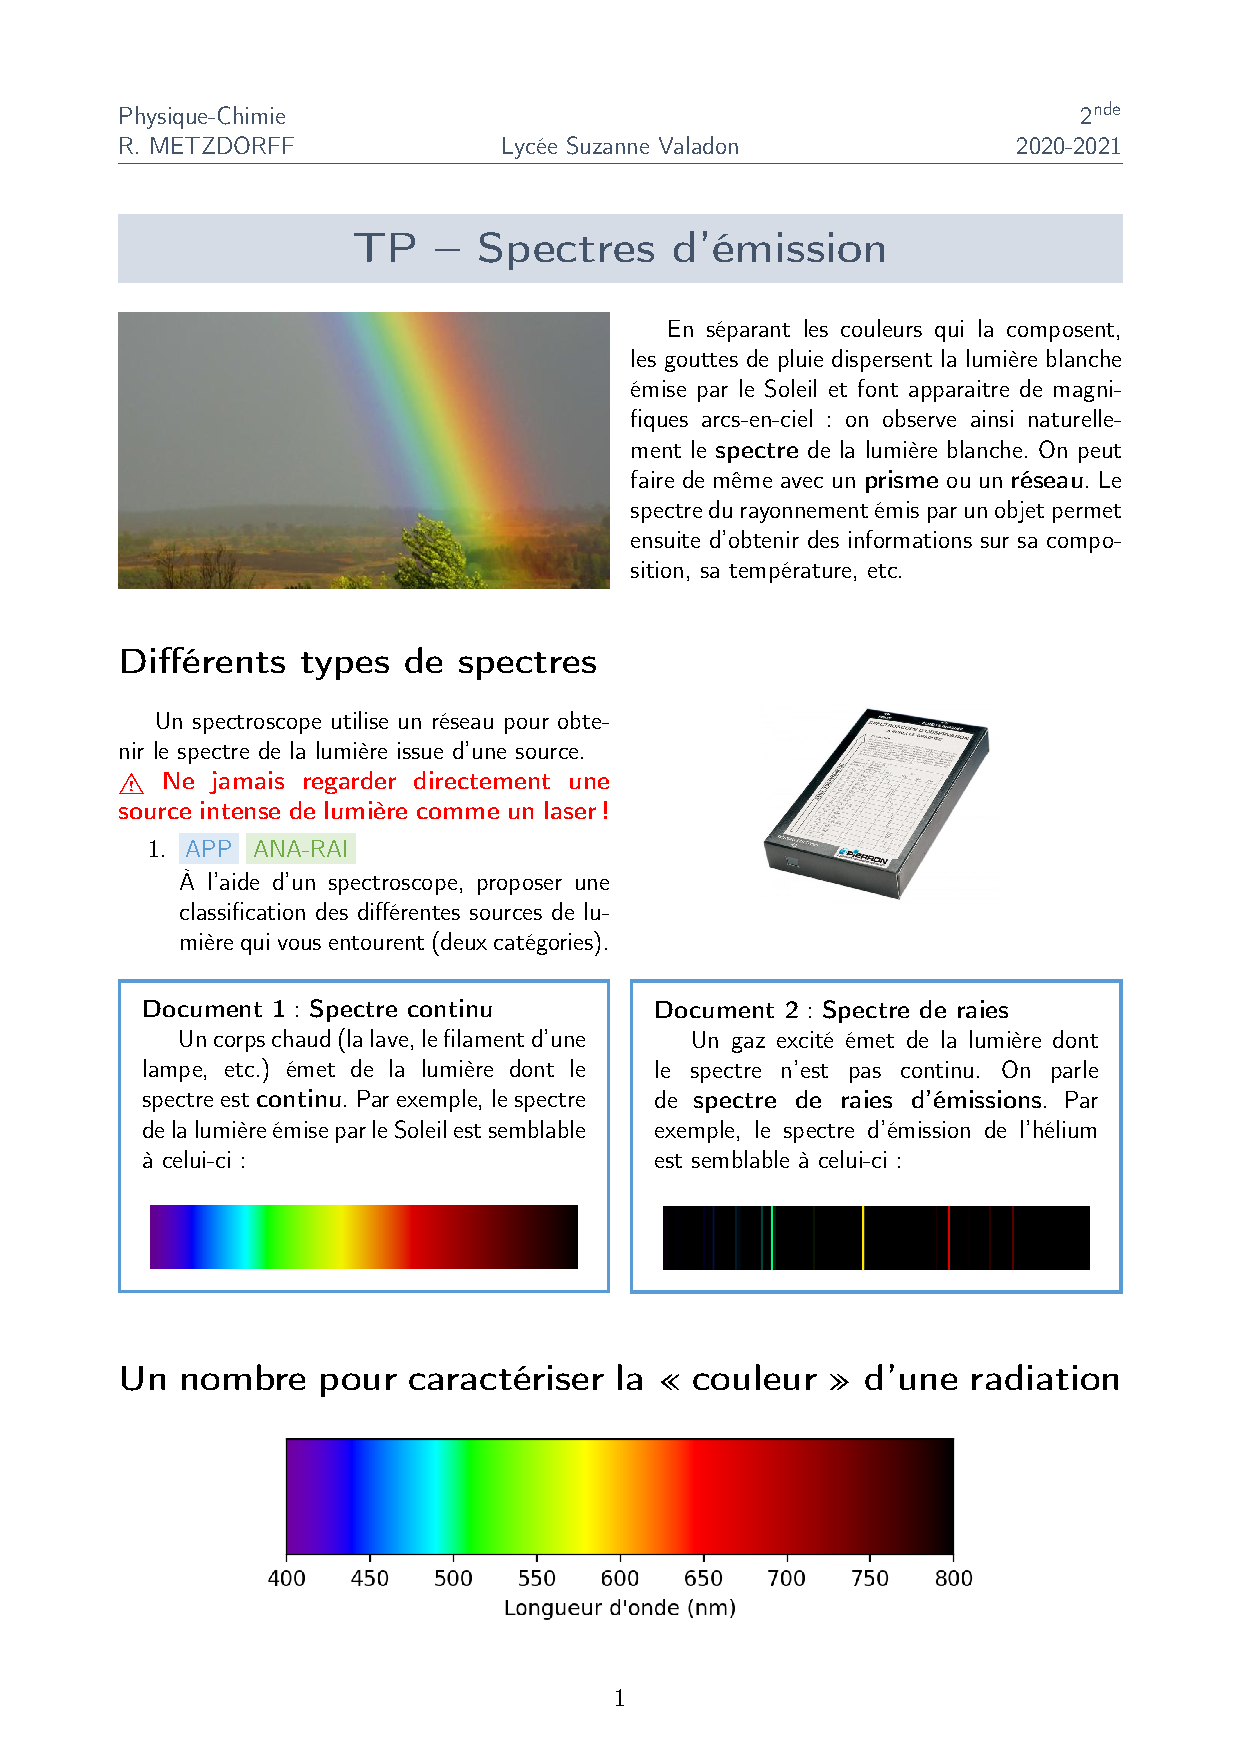
\includepdf[pages=-]{tp_spectre.pdf}

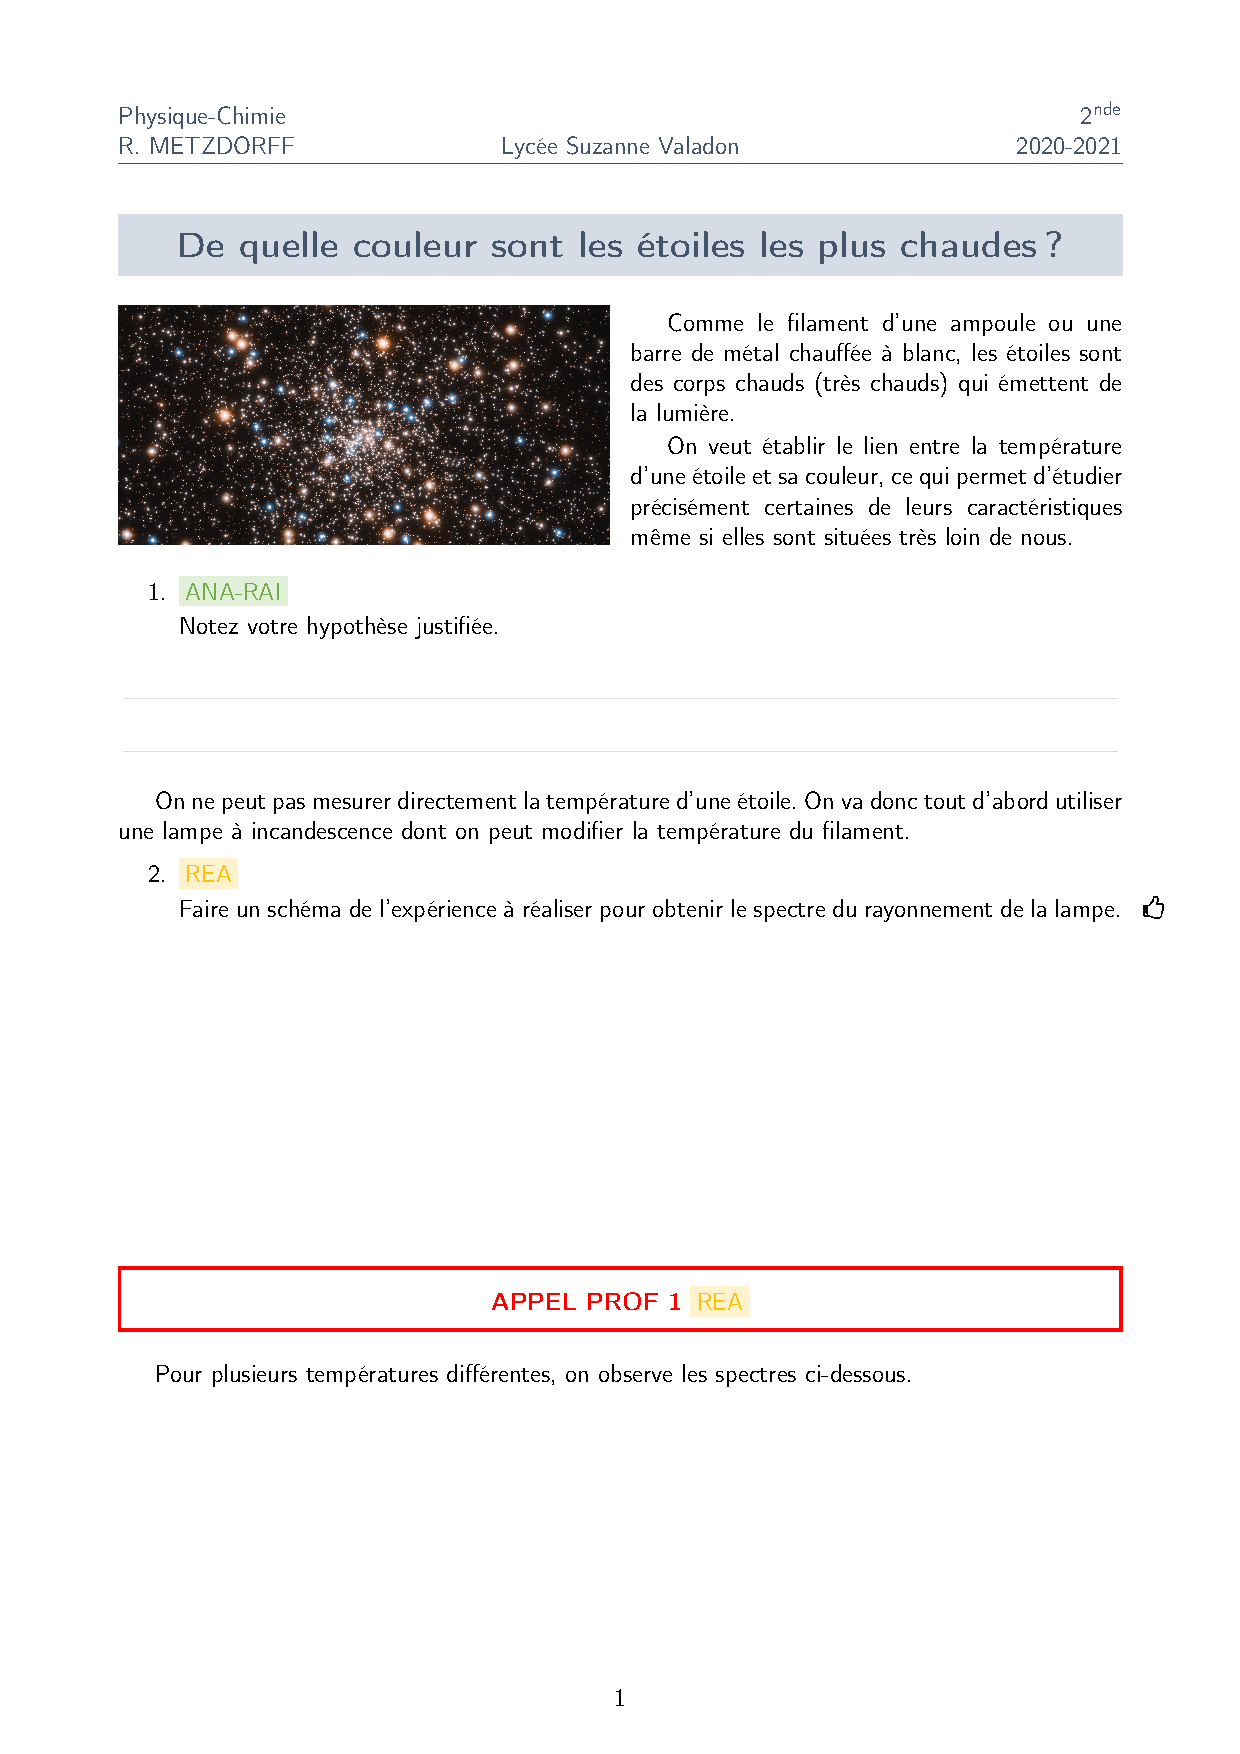
\includepdf[pages=-]{chap9_act_spectre_etoiles.pdf}

\begin{landscape}

\section*{Version 1}

\begin{center}
\begin{multicols}{3}

\includegraphics[width=\linewidth]{images/spectrum_black_body_temp3000K_notemp.png}


\includegraphics[width=\linewidth]{images/spectrum_black_body_temp5000K_notemp.png}


\includegraphics[width=\linewidth]{images/spectrum_black_body_temp10000K_notemp.png}
\end{multicols}

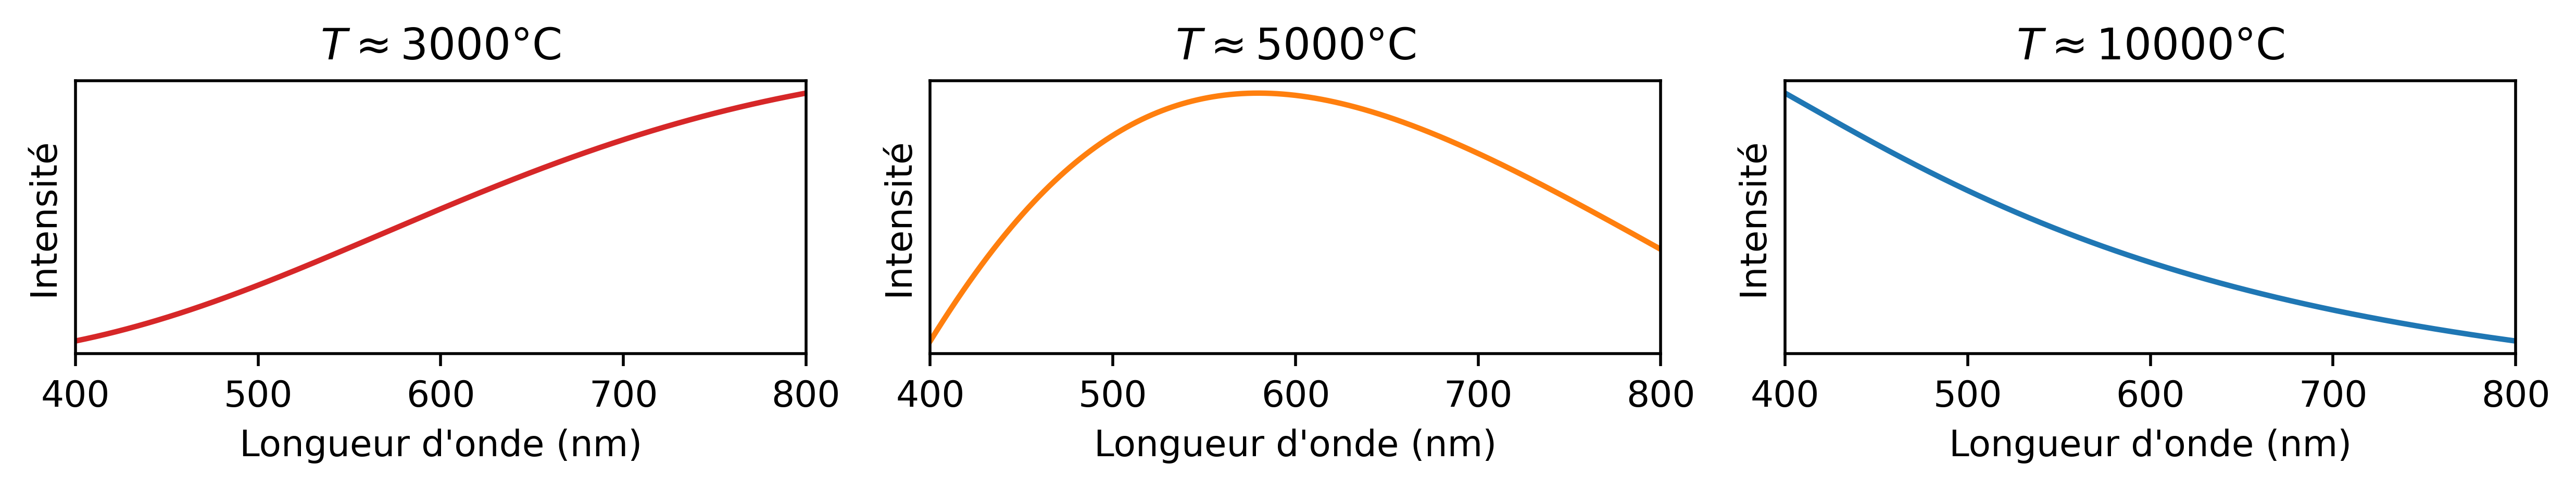
\includegraphics[width=\linewidth]{images/spectrum_black_body_curve10000K.png}
\end{center}

\section*{Version 2}

\begin{center}
\begin{multicols}{3}

\includegraphics[width=\linewidth]{images/spectrum_black_body_temp3000K.png}


\includegraphics[width=\linewidth]{images/spectrum_black_body_temp5000K.png}


\includegraphics[width=\linewidth]{images/spectrum_black_body_temp10000K.png}
\end{multicols}
\end{center}

\section*{Données}

\begin{center}
\begin{tabular}{l|c}
\textbf{Étoile} & \textbf{Température (\celsius)} \\
\hline
\hline
Proxima du Centaure	& 2\,700 \\
Tau Ceti							& 5\,000 \\
Rigel								& 11\,000 \\
\end{tabular}
\end{center}
\end{landscape}

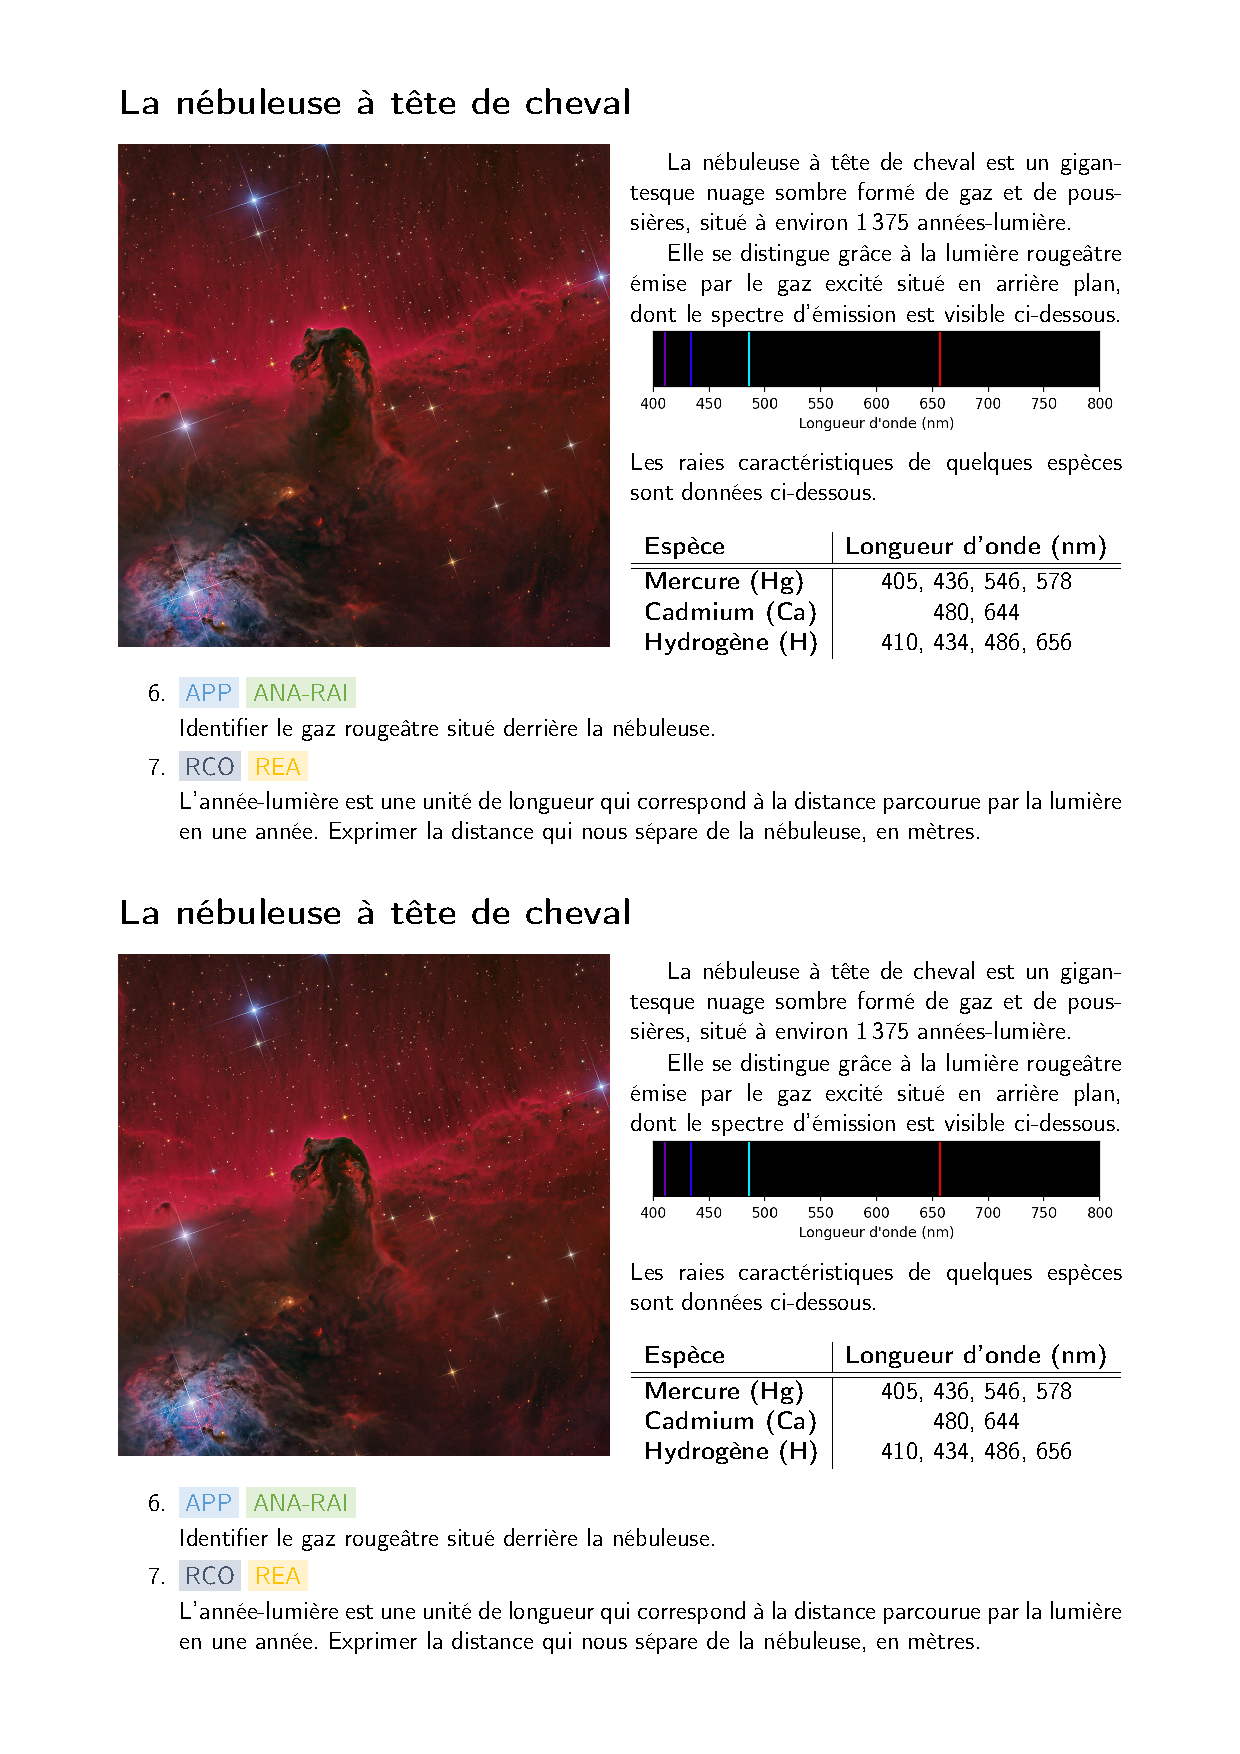
\includepdf[pages=-]{chap9_act_spectre_supp.pdf}

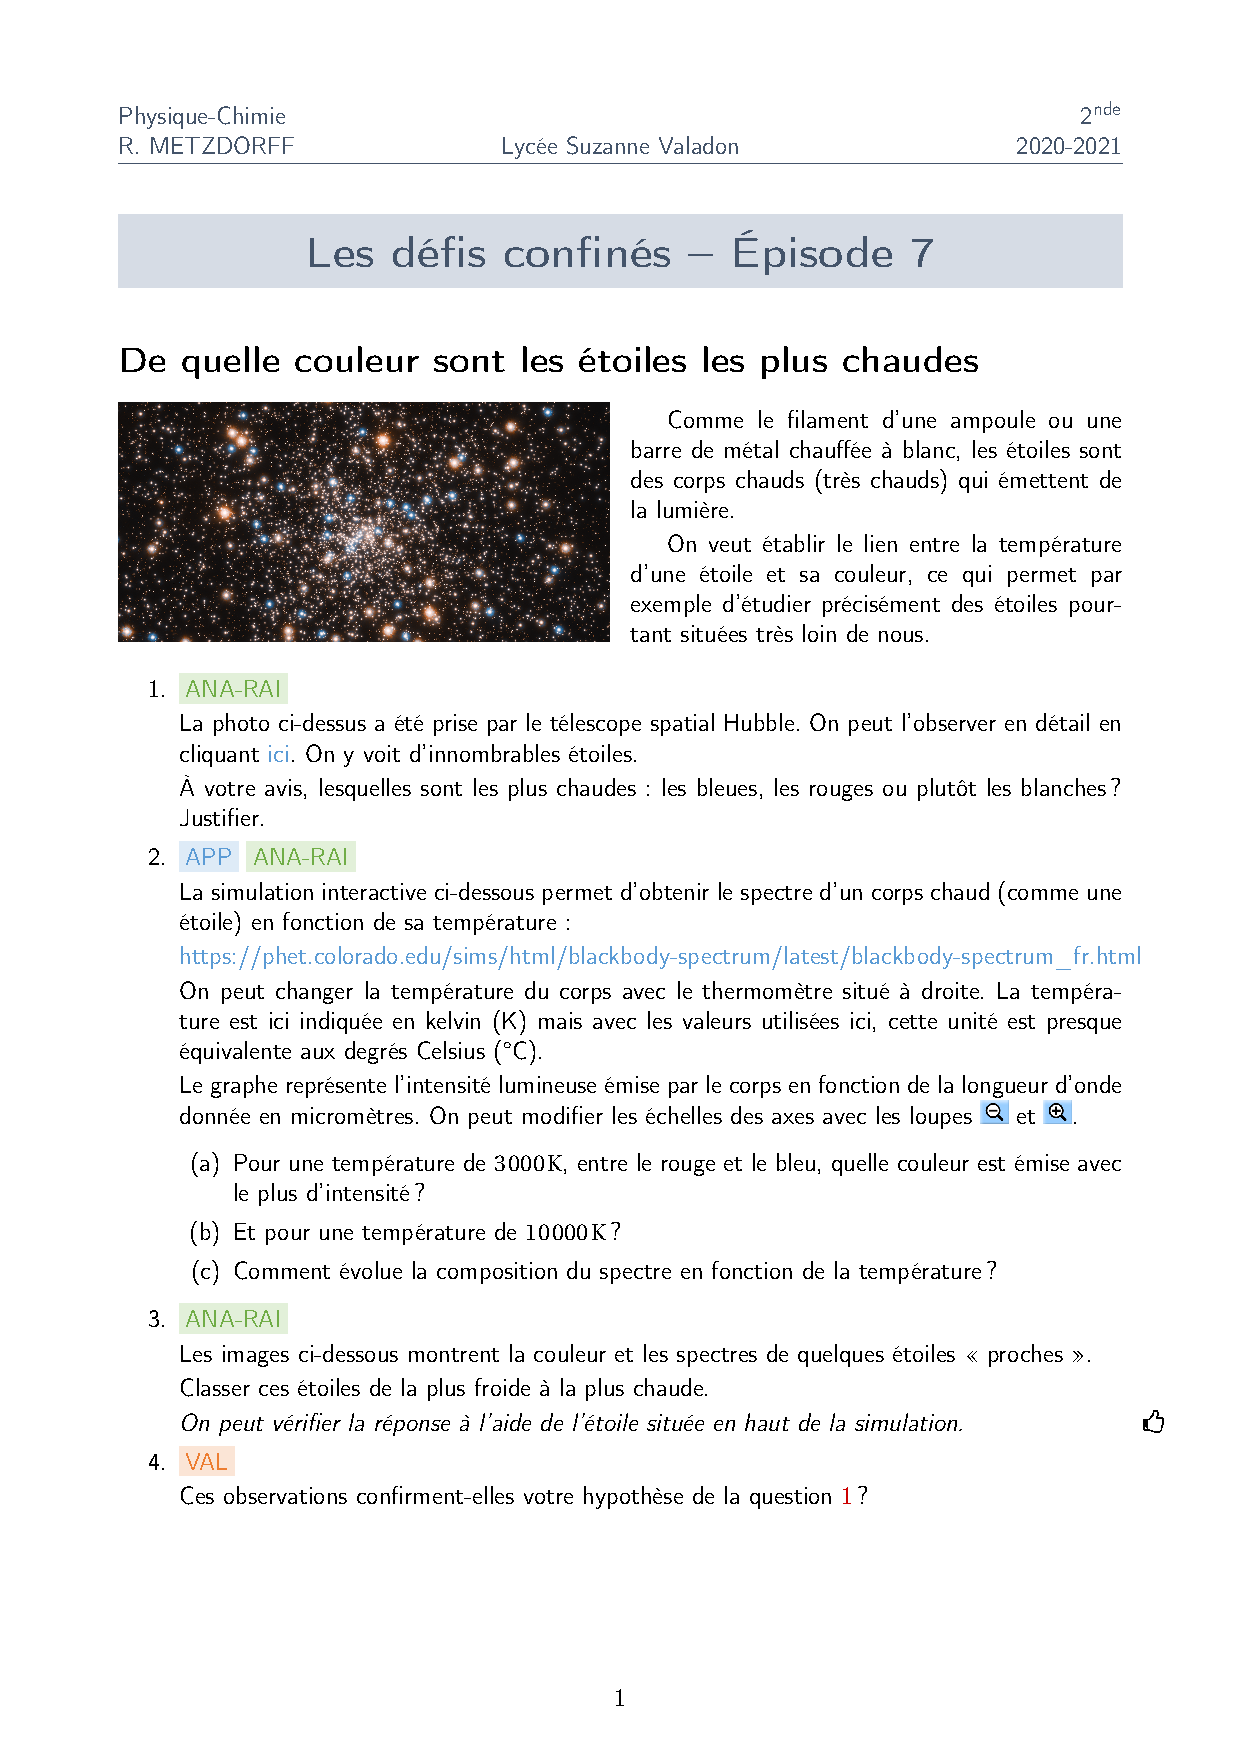
\includepdf[pages=-]{chap9_defis_confines_7.pdf}

\end{document}